\documentclass[10pt,a4paper]{article}
\usepackage[utf8]{inputenc}
\usepackage[english]{babel}
\usepackage{graphicx}
\usepackage{lmodern}
\usepackage{kpfonts}
\usepackage[left=2cm,right=2cm,top=2cm,bottom=2cm]{geometry}
\usepackage[export]{adjustbox}
\usepackage{dsfont}
\usepackage[noend]{algpseudocode}
\usepackage{wrapfig}
\usepackage{subcaption}
\usepackage{algorithm}
\newtheorem{lemma}{Lemma}
\newtheorem{definition}{Definition}
\newtheorem{notation}{Notation}
\newtheorem{proof}{Proof}
\author{Megi Dervishi}
\title{Algorithms and Programation}

\begin{document}

\maketitle
\section*{Homework 3 (4/12/2019)}
\subsection*{Exercise 1}
\subsection*{Solution}
The algorithm is not correct and we show this by the following counter-example.
Let us take the following graph which has initially $id = [0,1,2,3]$. We iterate over $i,j$ and apply the algorithm $UNION(i,j)$.
\begin{center}
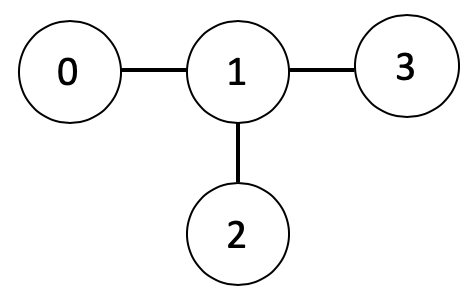
\includegraphics[width=0.25\textwidth]{graph.png}
\end{center}
When $i = 0$ and $j = 1$, we have that $id = [1,1,2,3]$. Until now the algorithm is correct. But when $i = 0$ and $ j = 2 $ we have: find($0$) $\neq$ find($2$)  so we go into the loop where we get a contradiction:
\begin{itemize}
\item \textbf{k = 0}
\begin{center}
  $ id[0] = id[0] \Rightarrow id = [2,1,2,3]$
\end{center}
\item \textbf{k = 1}
$$ \mathbf{id[1] \neq id[0]}$$ Therefore we do not go into the "if" and we finish with $id = [2,1,2,3]$ which is a mistake, because node $0,1,2$ should have the same root.

\end{itemize}
\subsection*{Exercise 2}
\subsection*{Solution}
\textbf{(1)}\\ We first show that if $G$ has distinct edges then there exists one unique MST. Let us assume by contradiction that $\exists T'$ MST such that $T \neq T'$.Therefore, without loss of generality, there is at least one edge of the graph $G$ such that $e \in T$ but $e\not\in T'$ and  $w(e) < w(e'), \, \forall e' \in T \cup T'$ (inequality is strict as edge weights are distinct). Since $T'$ is MST then $\{e\} \cup T'$ would create a cycle. In this cycle there exists at least one edge i.e $f$ such that $f \not\in T$ as that would make $T$ cyclic. By construction we have that $w(e) < w(f)$ since $e,f$ are distinct. If we replace $f$ with $e$ in $T'$ then we have created a spanning tree which has a smaller total weight than $T'$. Contradiction!\\\\
As for the second point we can observe that $\exists T', \, T''$ such that $w(T') = w(T'')$ and $T' \neq T''$ i.e. the second-best MST is not unique.
\begin{center}
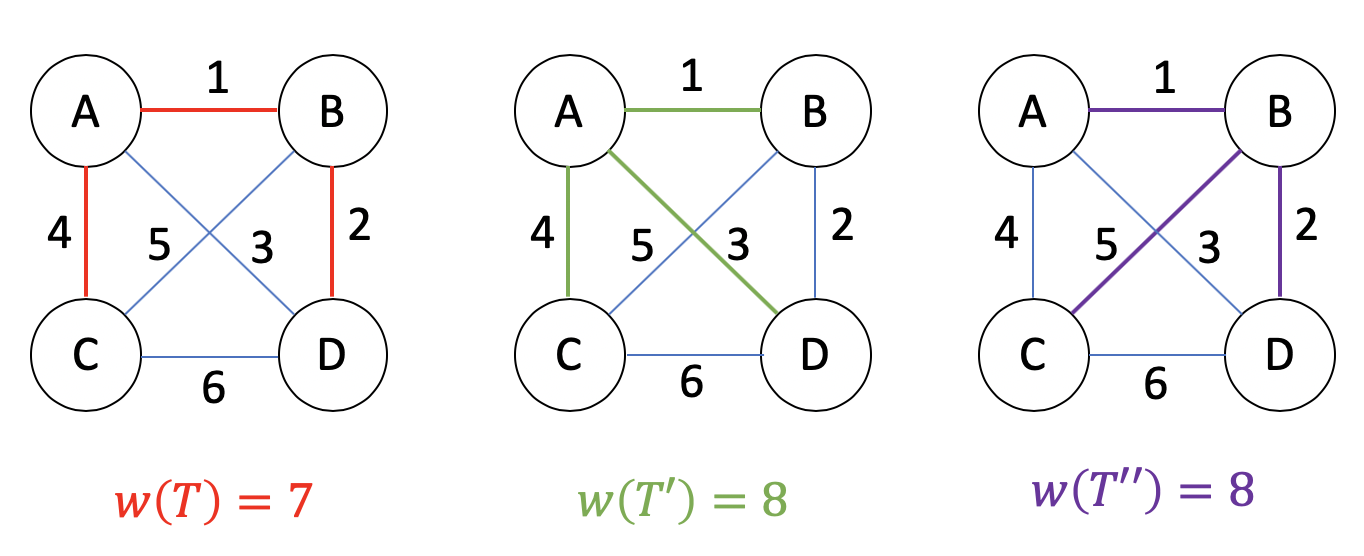
\includegraphics[width = 0.5\textwidth]{mst}
\end{center}
\textbf{(2)} \\
The theorem claims that there exists a second best MST that differs by one edge from the MST. We will prove a stronger theorem which states that all second best MST differ by exactly one edge from the MST. \\ 
By contradiction we assume	that there exists a second best MST, call it $T'$, such that $card (T \setminus T') \geq 2$, where $T$ is the MST of graph $G$.\\
\textbf{Note:} In this proof all inequalities involving weights are strict as edge weights are distinct.\\

Let $e \in T$ but $e \not\in T'$ such that $w(e) < w(u), \forall u \in T \setminus T'$ (this exists since all weight edges are distinct). If we add $e$ in $T'$ then that would create a cycle. In this cycle there exists an edge $f$ such that $f \in T'$ but $f \not\in T$, (this is possible because otherwise there would be a cycle in $T$). We want to prove that $w(e) < w(f)$. \\

We assume by contradiction that $w(f) < w(e)$. If we add $f$ in $T$ then that would create a cycle. In this cycle there exists an edge $g$ such that $g \in T$ but $g \not\in T'$. If we delete $g$ from the tree we have created a new spanning tree $T'' = T\setminus \{g\} \cup \{f\}$. Since $T$ is the MST to not have a contradiction we need $w(g) < w(f)$. So we have that $w(g) < w(f)< w(e) \Rightarrow w(g) < w(e)$. But we chose $e$ such that it is the edge in $T$ but not in $T'$ with the minimum weight. Contradiction!\\

So $w(e) < w(f)$. If we delete $f$ from $T'$ and add $e$ we have created a new spanning tree $T'' = T'\setminus \{f\} \cup \{e\} $ such that the general weight of $T''$ is strictly smaller than that of $T$ and $T''$ differs from $T$ by at least one edge ($T'' \neq T$). This means $T''$ is a second best MST with weight strictly smaller than $T'$. Contradiction!\\

Therefore we have proved by contradiction that all second best MST differ from the MST by exactly one edge. \\\\
\textbf{(3)}\\
We start our algorithm by creating a table $max$ which is of size $|V| \times |V|$ initializing everything to $None$. Since we are allowed the complexity $\mathcal{O}(|V|^2)$ then our algorithm can simply traverse on all vertices $u$ and $v$ of $T$(spanning tree) by finding what is the smallest weighted edge between the path of $u$ and $v$ using BFS. Let $Q$ be a queue initialized as empty. The function $Q.$\textbf{append}$(u)$ adds $u$ from the "bottom" of $Q$ whereas $Q.$\textbf{pop}()
deletes the first element of $Q$ and returns is. Also the function $\mathbf{Neighb}(T,x)$ finds the neighbours of vertex $x$ in tree $T$.

\begin{algorithm}
\begin{algorithmic}[1]
\Function{Compute\_max\_table ($T$)}{}
	\For {$u \in T.Verteces$} 
		\For {$v \in T.Verteces$}
			\State $max[ u,v] \gets None$ 
		\EndFor
		\State $Q \gets []$
		\State $Q.$\textbf{append}$(u)$
		\While {$length (Q) > 0 $}{
			\State $x =Q.$\textbf{pop}$()$
			\For { $x \in \mathbf{Neighb}(T,x)$}
				\If {$max[u,v] \neq None \land u \neq v$}
					\If {$w(x,v) > w(max[u,x])  \lor x = u$} 
						\State $max[u,v] = (x,v)$
					\Else {}
						\State $max[u,v] = max[u,x]$
					\EndIf
					\State $Q.$\textbf{append}$(v)$
				\EndIf
			\EndFor	
		}
		\EndWhile	
	\EndFor
	\Return $max$
\EndFunction
\end{algorithmic}
\end{algorithm}

\textbf{Proof of Correctness}\\
We prove the algorithm using induction.\\
Basic case: Trivial ( $|V| = 1$, $|E| = |V| -1 = 0$, $max[u,u] = None$.)\\
Induction case: Let us assume that the algorithm is correct i.e. we have computed the $max$ table for all $n$-verteces in $T$. We want to show that it is correct for $n+1$ - verteces. Let us add a new vertex $k$ in $T$. Since $T$ is a spanning tree and $T \cup \{k\}$ needs also to be a spanning tree i.e. no cycle then $k$ has one neighbour call it $ p_k \in T.Verteces$. Then we know that the path of $u  \rightarrow k$ for all $u \in T.Verteces$ is the same as the path of $u \rightarrow p_k$ and $p_k \rightarrow k$. By induction hypothesis we know what is the $max[u,p_k],\, \forall u \in T.Verteces$ then what the algorithm asks us to check is two cases:\\
1. If $w((p_k,k)) > w(max(u,p_k))$ then we replace the $max[u,p_k]$ by $(p_k,k)$ which makes sense since the maximum weighted edge for the path ($u,p_k$) would be $(p_k,k)$\\
2. If it is smaller then $max[u,k]= (u,p_k)$. \\
So by induction we can correctly compute the $max$ table for all verteces in $T$.\\

\textbf{Complexity}\\
If we construct $T$ as a dictionary then finding the neighbour verteces of $x$( $\mathbf{Neighb}(T,x)$) is done in $\mathcal{O}(1)$ - time. The BFS is of time-complexity $\mathcal{O}(|V| + |E|)$ and we perform that on all verteces $V$ so we get $\mathcal{O}(|V|(|V|+|E|))$. Since for spanning trees $|E| = |V|-1$ then the time-complexity for this algorithm is $\mathcal {O}(|V|^2)$. 
The space complexity is also $\mathcal{O}(|V|^2)$ since it is the space required to create the table $max$ and store $T$. \\\\
\textbf{(4)}\\
To create this algorithm we shall use the stronger theorem of part $(b)$ i.e. a second best MST differs from MST by exactly one edge. \\
First our algorithm needs to compute a MST which by the Prim's algorithm using Fibonacci heaps takes time-complexity $\mathcal{O}(|E| +| V|\log| V|) )$(as stated during the lecture). Having computed a MST then we should create/compute the $max$ table for the MST which is done in $\mathcal{O}(|V^2|)$ time. \\
Now we want to find the edge $f \in G\setminus T$ which will replace an edge $e \in T$  to create a new spanning tree $T'$ such that $w(T') = w(T) - w(e) + w(f)$ will be minimized. If we assume we have $f$ the edge $e$ that will minimize the most $w(T')$ would be $max[f]$ (by abuse of notation) i.e. the value in the $max$ table of the unique path in $T$ between the verteces that create edge $f$. So our algorithm has to simply iterate over all the edges $k \in G \setminus T.Edges$ and check if $val = w(max[k]) - w(k)) < curr$, where $curr$ is simply a variable to keep track of the minimal weight of $T'$. If the condition is true then we replace $curr$ by $val $ and $f = k$ ($f$ is also a variable outside the loop to keep track of the edge). After we have traverse all the edges then we are sure that we have found the edge $f$ which would give us the second best minimal weighted spanning tree i.e. second best MST (algorithm is correct).  In the end of the algorithm we would return the tree $T' = T \setminus \{max[f]\} \cup \{f\}$. \\
Since $max$ is a table then finding $max[k]$ and computing $val$ is done in $\mathcal{O}(1)$. Also traversing through all the edges assuming that $|E|$ is bounded above by $|V|^2$ then we have that the time complexity for this algorithm is $O(|V|^2)$. The space complexity is the also $O(|V|^2)$ since it is the space required to create the table $max$.

\break
\subsection*{Exercise 3}
\subsection*{Solution}

\textbf{(1)}\\
As soon as you have $k$ matching edges you get k pairs of vertices i.e. $2k$ vertices that are connected. This means that if we choose one of these $2k$ vertices  to be in the maximum independent set of $G$ then its adjecent vertex will not be part of it. Hence from $2k$ vertices we can include at most $k$ vertices in the set. Therefore from $2n$ total vertices and a maximum matching set of cardinality $k$ we are left at most with $2n - k$ vertices that can be in the maximum independent set.\\\\
\textbf{(2)}\\
In this proof of correctness we want to prove that the RED set is the maximum independent set. To do so we can use question (1): If an independent set is of cardinality $2l-k$ then it is a maximum independent set where $2l$ is the number of vertices of $G$. So we start by proving the invariant: "The RED set is an independent set". The algorithm has three stages/cases: before the loop, during the loop and after the loop in which the RED set is changed and we want to prove that after these changes the invariant stays true.\\ 
We introduce the following notations/definitions:
\begin{itemize}
\item $G.E, \, G.V$ denotes the set of edges and vertices respectively of the graph $G$
\item $c(v) = R, \, c(v) = B, \, c(v) = W$ denotes the color of vertex $v$ to be Red($R$), Blue($B$) and Uncolored($W$).
\item $M_E$ is the set of edges in the maximum matching set which has size $k$
\item $M_V$ is the set of vertices in the maximum matching set which has size $2k$
\item $(u,v) \in M_E \Rightarrow u,v \in M_V$, where $(u,v)$ is the edge of vertices $u,v$
\item $u \in M_V \Rightarrow \exists p \in M_V\setminus \{u\} \,\text{ st } \,(u,p) \in M_E$
\item $U, V$ have $l$ vertices (we use $n$ in the proofs so as to not confuse it with the cardinality of $U,V$).
\item $u,v$ are said to be neighbours if there exists an edge that connects them.
\end{itemize}
We also will need the following lemma:
\begin{lemma} If $u,v \not \in M_V$ and $(u,v) \in G.E$ then $M_E \cup \{(u,v)\}$ is a matching set.
\end{lemma}
\textbf{Proof}\\
Suppose by contradiction that $M_E \cup \{(u,v)\}$ is not a matching set then there must exists an edge $e$ that creates a conflict with $(u,v)$. This means that $e$ and $(u,v)$ must share a vertex, which implies that either $u$ or $v$ are in $M_V$. Contradiction!\\\\ 
\textbf{Before the loop}\\
In this stage we color in red the verteces which are not in $M_V$. In other words: "If $u \not\in M_V$ and $v \not\in M_V$ then $u,v$ are not neighbours" where $u,v$ are vertices outside the $k$-matching set, and that we want to color red. If $u,v$ are colored red and they aren't neighbours then they are independent so by adding them to the RED set we will not have any conflicts in the set i.e. the invariant will still be true.
Now we want to prove the proposition which can be done by contrapositive:
\begin{center}
"If $u,v$ are neighbours then $u$ or $v$ must be in $M_V$"
\end{center} 
Assuming $u,v$ are neighbours then there exists an edge $(u,v)$ that connects them. 
If $(u,v) \in M_E$ then we are done since both vertices are in $M_V$ by definition. If $(u,v) \not\in M_E$ then we want to prove that $u$ or $v$ is in $M_V$. Suppose by contradiction that $u$ and $v$ are not in $M_V$. Then applying Lemma 1 there aren't any conflicts in $M_E$ if we add the edge $(u,v)$. But now we have created a larger matching set, $\{(u,v)\} \cup M_E$. Contradiction!\\
So if $(u,v) \not\in M_E$ then $u$ or $v$ must be in $M_V$. By contrapositive we have concluded the proof for case 1 i.e. the RED set before the loop is still an independent set. \\\\
\textbf{During the loop}\\
In this stage we shall prove the invariant for 1 iteration of the loop and by repetition/induction that will be true for all iterations of the loop. We assume that before the loop the RED set is independent as we proved in stage 1. Also now we have colored in red all the vertices that are not in $M_V$ i.e. all the following uncolored vertices are in $M_V$. The while loop starts by the following condition: 
\begin{center}
"$\exists u \in M_V \text{ st } \, c(u) = W\,\, \land \, \, \exists r \in \text{ RED  st  } (u,r)\in G.E$"
\end{center}
If this condition is not true then the RED set is not changed and we skip to stage 3 i.e. the invariant stays true.
Otherwise we set $c(u) = B$ and by definition since $u \in M_V$ there exists $v \in M_V \setminus \{u\}$ such that $(u,v) \in M_E$. We want to color $v$ red so we have to make sure that $v \in $ RED won't create any conflicts with all the other red vertices. By contradiction suppose that $\exists p \in $ RED st $(p,v) \in G.E$. Without loss of generality we take $v,r \in V$ and $p,u \in U$. Now we look at the four possible cases which are ilustrated by the below figures: 
\begin{figure*}[h!]
\centering
    \begin{subfigure}[t]{0.5\textwidth}
        \centering
        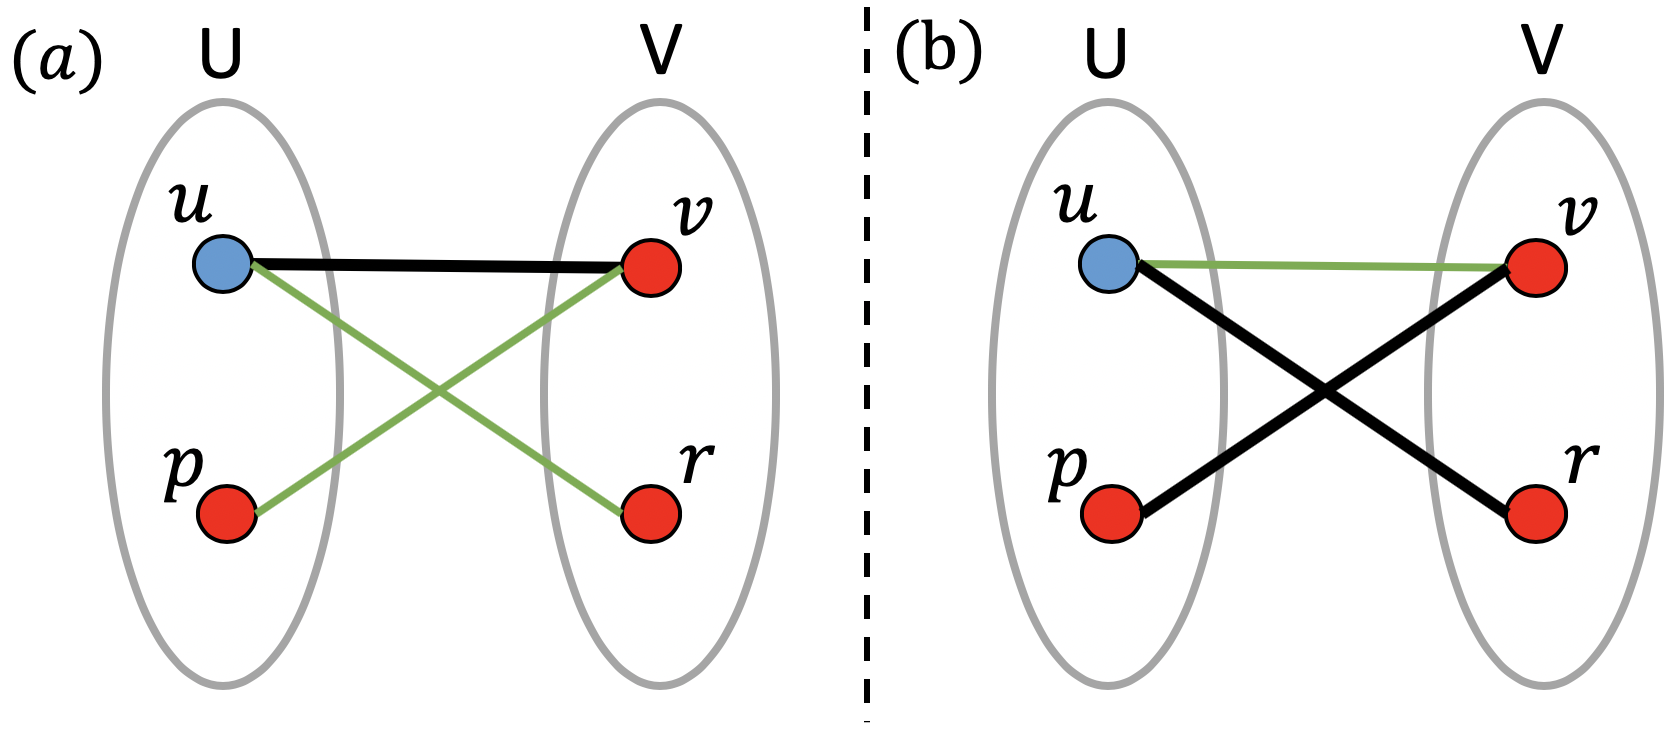
\includegraphics[width = \textwidth]{case_1}
        \caption*{ \textbf{Case 1}}
    \end{subfigure}%
    ~ 
    \begin{subfigure}[t]{0.5\textwidth}
        \centering
        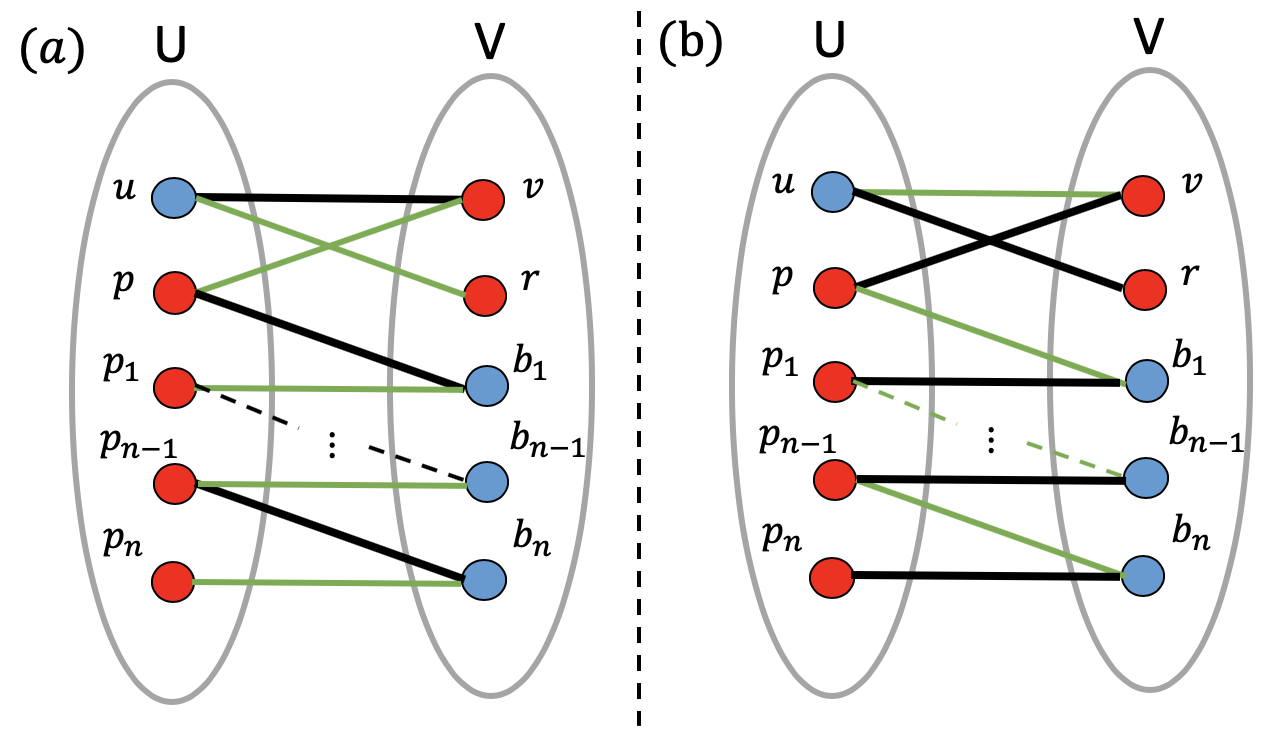
\includegraphics[width = 0.8\textwidth]{case_2}
        \caption*{\textbf{Case 2 (3)}}
    \end{subfigure}
    \begin{subfigure}[t]{0.5\textwidth}
        \centering
        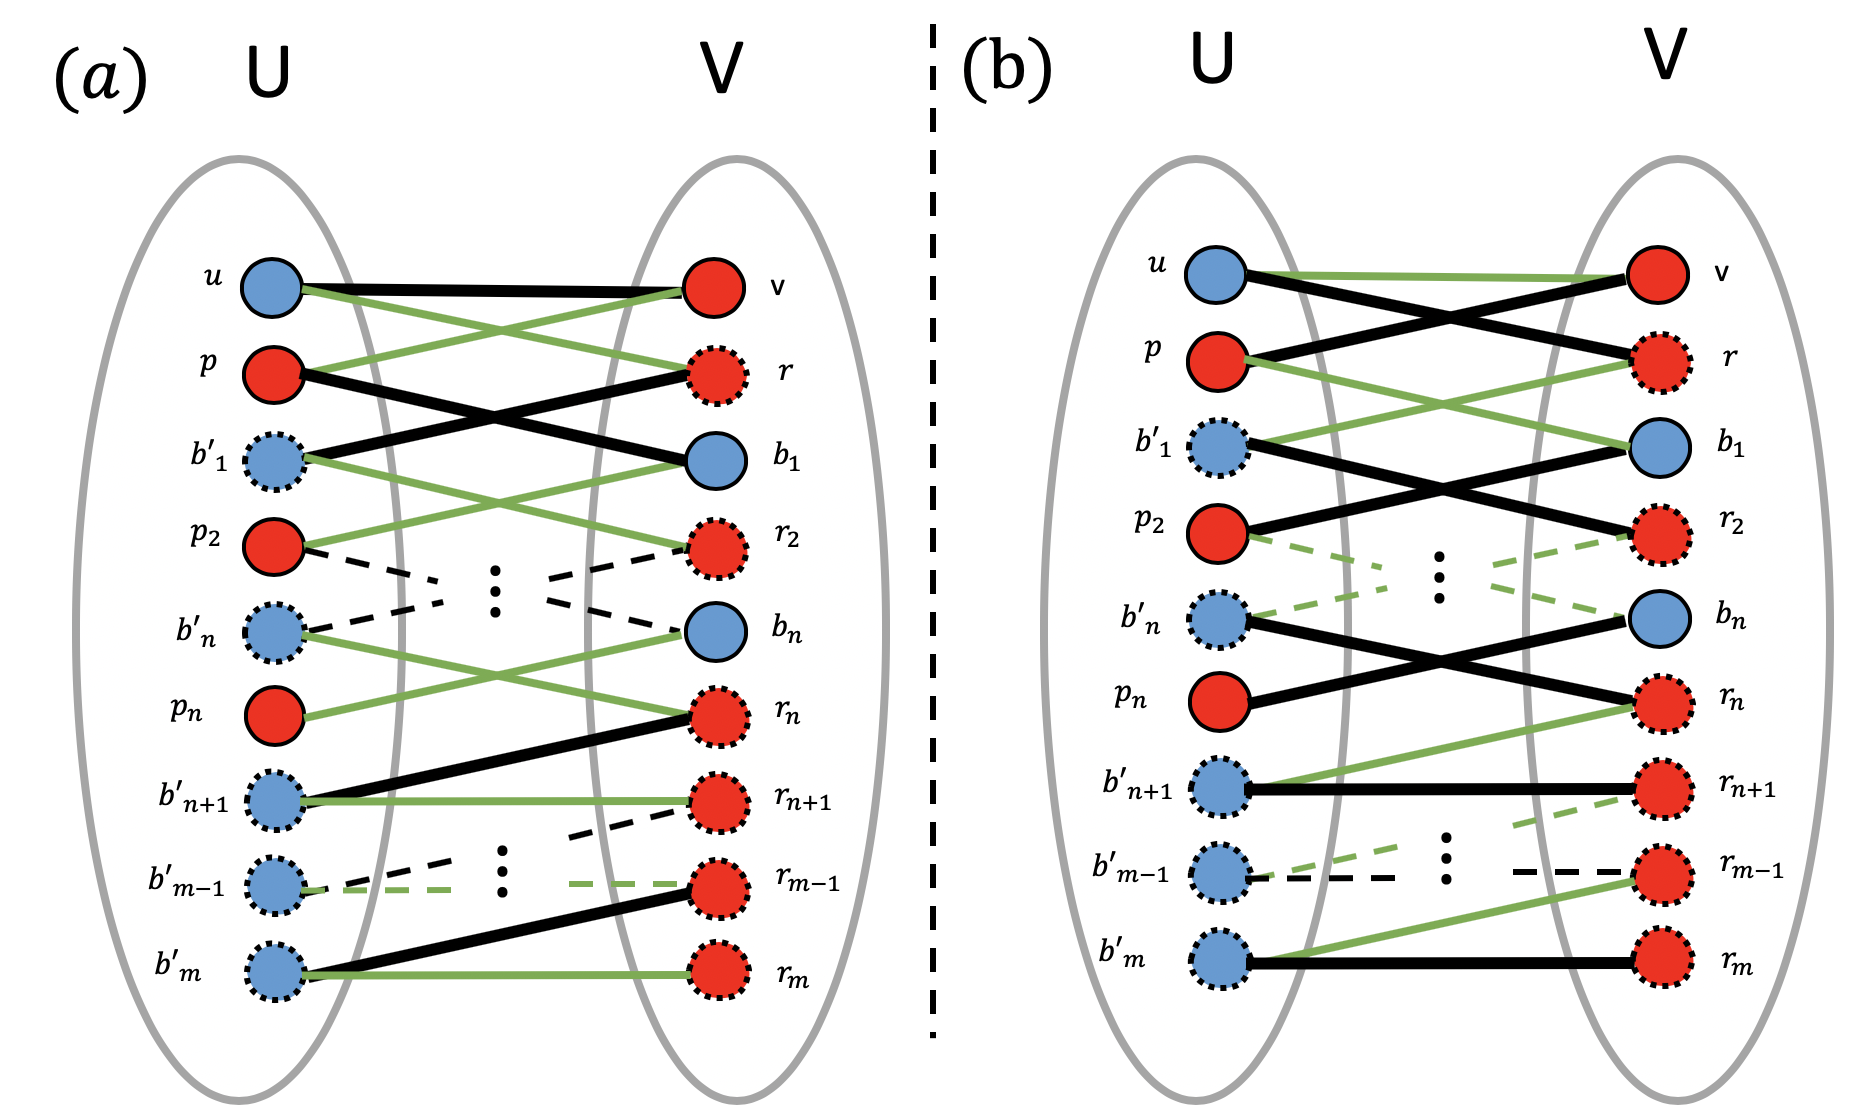
\includegraphics[width = 0.9\textwidth]{case_4}
        \caption*{\textbf{Case 4}}
    \end{subfigure}
    ~ 
    \caption{ Diagram of vertices of interest for the contradiction proofs of case 1, 2(3) and 4.  Figures (a) of each case represent the current disposition of $M_E$ with the contradiction hypothesis ($c(v) = R, c(p) = R, (v,p)\in G.E$). Figures (b) show how this extra edge leads to a contradiction. Black edges are matching edges; Green edges are not matching edges; The color of the vertices represent which set they belong to; In case 4 the doted/solid vertices are used to separate the two zig-zags. }
\end{figure*} 

\begin{enumerate}
\item $\mathbf{p \not \in M_V \, \land \, r\not\in M_V}$\\
Figure 1, case 1 (a) illustrate a part of the bipartite graph in which we assume that there exists an edge $(p,v) \in G.E$, $c(v) = R$ and $(u,v) \in M_E$. Since $p,r$ are not in $M_V$ using lemma 1, we are sure there won't be any conflicts if we were to add in $M_E$ the edges $(p,v), (u,r)$ instead of the edge $(u,v)$. But that means we have just created a larger matching set, $M_E\setminus \{(u,v)\} \cup \{(p,v),(u,r)\}$. Contradiction! So for this case it is impossible for edge $(p,v)$ to exist in the edges of the graph $G$.

\item $\mathbf{p \in M_V \, \land \, r\not\in M_V}$   and    $\mathbf{r \in M_V \, \land \, p\not\in M_V}$  \\
The two cases are in fact symmetric so for simplicity we prove the contradiction for one of them. Since $p \in M_V$ and $c(p) = R$ then that means $\exists b_1$ such that $c(b_1) = B, (b_1, p) \in M_E$ and $\exists p_1 $ such that $ (b_1, p_1) \in G.E$. We inductively repeat the following reasoning on $p_i$ until it terminates with a vertex $p_n$ which is in RED but not in $M_V$. The graph can be seen summarized in Figure 1, case 2 (a). As we observe in the figure we have $M_E$ edges in between $p_{i-1}$ and $b_i$ for $i \in [1,n] \cap \mathbb{N}$. Therefore we have a total of $n + 1$ matching edges,  $n$-edges in the zigzag plus the $(u,v)$ edge. 
Now we remove these edges from $M_E$ and consequently their vertices from $M_V$ which assures that there won't be any conflict when we add the following edges (by lemma 1):  $(p_{i},b_i)$ where $i \in  [1,n] \cap \mathbb{N}$. This makes the cardinality of this part of $M_E$ equal to $n$ plus the two edges $(p,v), (u,r)$. We have created a larger $M_E$:
$$
M_E \cup \underbrace{\{ (p_i, b_i) | i \in [1, n] \cap \mathbb{N}  \} \cup \{(p,v), (u,r)\}}_{\text{Cardinality of } n + 2} \setminus \underbrace{\{ (p_{i-1}, b_i) | i \in [1, n] \cap \mathbb{N} \}}_{\text{Cardinality of } n + 1}
$$
Contradiction!
\break
\item $\mathbf{p \in M_V \, \land \, r\in M_V}$\\
Following the same reasoning as in the previous case we inductively create the following zigzags which will terminate at a certain $p_n, r_m \not\in M_v$, the summary of which is shown in Figure 1, case 4.
We denote by $p_i$ and $b_i$ the red and blue vertices respectively for the zigzag starting from $p = p_0$ and we denote $r_i, b'_i$ the red and blue vertices for the zig-zag starting from $r = r_0$.  The edges in $M_E$ have the following indices:\\ 1) first zigzag $(p_{i-1}, b_i)$\\ 2) second zigzag $(r_{j - 1}, b'_j)$\\ for $i \in [1, n] \cap \mathbb{N}$ and $j \in [1, m] \cap \mathbb{N}$. With the edge $(u,v) \in M_E$, the cardinality of this part of the $M_E$ is $n+m+1$. Now we remove all these edges from the $M_E$ and consequently their vertices from the $M_V$ and add a different combination of them that will not create any conflicts (by Lemma 1) because the added edges do not share vertices and their vertices are not in $M_V$. We add:\\
1) first zigzag $(p_i, b_i)$\\
2) second zigzag $(r_j, b'_j)$\\
for $i \in [1, n] \cap \mathbb{N} $ and $j \in [1, m] \cap \mathbb{N}$. Furthermore we can add $(u,r)$ and $(v,p) $ which brings the cardinality of this part of the $M_E$ to $n+m+2$. We have just created a larger matching set:
$$
M_E \cup \underbrace{\{ (p_i, b_i), (r_j, b'_j) | i,j \in [1, n]\times [1, m] \cap \mathbb{N}^2 \} \cup \{(p,v), (u,r)\}}_{\text{Cardinality of } n + m + 2} \setminus \underbrace{\{ (p_{i-1}, b_i), (r_{j - 1}, b'_j) | i,j \in [1, n] \times [1, m] \cap \mathbb{N}^2\}}_{\text{Cardinality of } n + m + 1}
$$
Contradiction! 

\end{enumerate}
By contradiction on the four cases we can conclude that it is impossible for the edge $(p,v)$ to exist so we can include the vertex $v$ in the set RED without causing any conflicts with the rest of the verteces already in the RED set. During the loop RED stays independent. \\\\
\textbf{After the loop}\\
After we have exited the loop the RED set is independent. Now we have to color the remaining vertices in $U$ in red and those in $V$ blue. It is possible that after the loop there are no remaining vertices so in that case we are done with the proof. Otherwise we continue: Note that we exit the loop when  there exists no edge connecting a red vertex with an uncolored vertex. So all the rest of vertices which were not yet colored if they were to be added in the set RED they will not create any conflicts. Of course we do not add all of them but we add the vertices which are in one of the parts of the graph i.e. U. Due to the property of a bipartite graph we are sure that the vertices in U will be independent within themselves as they only connect with vertices in V.\\ Hence by the end of this algorithm the RED set stays an independent set.\\\\

Now that we have shown that RED is an independent set, it is left to show that $card(\text{RED}) = 2l - k$. Since at the end of the algorithm all the vertices are colored it is easier to count the number of Blue vertices: One out of two of the $2k$ vertices of the $k$-matching edges is colored in blue (inside or outside the loop). Therefore we have $k$ blue vertices, which means that we are left with $2l-k$ red vertices where $2l$ is the number of vertices in the graph $G$.\\\\

Since RED is an independent set with a cardinality $2l-k$ then RED is the maximum independent set of $G$. The algorithm is correct! $\quad \quad \quad\quad\quad\quad \quad \quad\quad\quad\quad \quad \quad\quad \quad \quad\quad\quad \quad \quad\quad\quad\quad\quad\quad\quad \quad \quad\quad\quad\quad \quad \quad\quad\quad \textbf{QED}$

\end{document}